% !TEX TS-program = XeLaTeX
% use the following command:
% all document files must be coded in UTF-8
\documentclass[spanish]{textolivre}
% build HTML with: make4ht -e build.lua -c textolivre.cfg -x -u article "fn-in,svg,pic-align"

\journalname{Texto Livre}
\thevolume{15}
%\thenumber{1} % old template
\theyear{2022}
\receiveddate{\DTMdisplaydate{2022}{2}{5}{-1}} % YYYY MM DD
\accepteddate{\DTMdisplaydate{2022}{4}{24}{-1}}
\publisheddate{\DTMdisplaydate{2022}{5}{30}{-1}}
\corrauthor{Francisco Javier Rocha Estrada}
\articledoi{10.35699/1983-3652.2022.38234}
%\articleid{NNNN} % if the article ID is not the last 5 numbers of its DOI, provide it using \articleid{} commmand 
% list of available sesscions in the journal: articles, dossier, reports, essays, reviews, interviews, editorial
\articlesessionname{articles}
\runningauthor{Rocha Estrada y Rincón Flores}
%\editorname{Leonardo Araújo} % old template
\sectioneditorname{Hugo Heredia Ponce}
\layouteditorname{Carolina Garcia}

\title{Docentes universitarios frente al confinamiento académico: un análisis exploratorio}
\othertitle{Professores universitários enfrentando o confinamento acadêmico: uma análise exploratória}
\othertitle{University teachers facing academic lockdown: an exploratory analysis}
% if there is a third language title, add here:
%\othertitle{Artikelvorlage zur Einreichung beim Texto Livre Journal}

\author[1]{Francisco Javier Rocha Estrada \orcid{0000-0001-5583-6559} \thanks{Email: \url{fcojvr25@gmail.com}}}
\author[2]{Elvira Guadalupe Rincón Flores \orcid{0000-0001-5957-2335} \thanks{Email: \url{elvira.rincon@tec.mx}}}
\affil[1] {Tecnologico de Monterrey, Escuela de Humanidades y Educación, Monterrey, Nuevo León, México.}
\affil[2] {Tecnologico de Monterrey, Instituto para el Futuro de la Educación, Monterrey, Nuevo León, México.}


\addbibresource{article.bib}
% use biber instead of bibtex
% $ biber article

% used to create dummy text for the template file
\definecolor{dark-gray}{gray}{0.35} % color used to display dummy texts
\usepackage{lipsum}
\SetLipsumParListSurrounders{\colorlet{oldcolor}{.}\color{dark-gray}}{\color{oldcolor}}

% used here only to provide the XeLaTeX and BibTeX logos
\usepackage{hologo}

% if you use multirows in a table, include the multirow package
\usepackage{multirow}

% provides sidewaysfigure environment
\usepackage{rotating}

% CUSTOM EPIGRAPH - BEGIN 
%%% https://tex.stackexchange.com/questions/193178/specific-epigraph-style
\usepackage{epigraph}
\renewcommand\textflush{flushright}
\makeatletter
\newlength\epitextskip
\pretocmd{\@epitext}{\em}{}{}
\apptocmd{\@epitext}{\em}{}{}
\patchcmd{\epigraph}{\@epitext{#1}\\}{\@epitext{#1}\\[\epitextskip]}{}{}
\makeatother
\setlength\epigraphrule{0pt}
\setlength\epitextskip{0.5ex}
\setlength\epigraphwidth{.7\textwidth}
% CUSTOM EPIGRAPH - END

% LANGUAGE - BEGIN
% ARABIC
% for languages that use special fonts, you must provide the typeface that will be used
% \setotherlanguage{arabic}
% \newfontfamily\arabicfont[Script=Arabic]{Amiri}
% \newfontfamily\arabicfontsf[Script=Arabic]{Amiri}
% \newfontfamily\arabicfonttt[Script=Arabic]{Amiri}
%
% in the article, to add arabic text use: \textlang{arabic}{ ... }
%
% RUSSIAN
% for russian text we also need to define fonts with support for Cyrillic script
% \usepackage{fontspec}
% \setotherlanguage{russian}
% \newfontfamily\cyrillicfont{Times New Roman}
% \newfontfamily\cyrillicfontsf{Times New Roman}[Script=Cyrillic]
% \newfontfamily\cyrillicfonttt{Times New Roman}[Script=Cyrillic]
%
% in the text use \begin{russian} ... \end{russian}
% LANGUAGE - END

% EMOJIS - BEGIN
% to use emoticons in your manuscript
% https://stackoverflow.com/questions/190145/how-to-insert-emoticons-in-latex/57076064
% using font Symbola, which has full support
% the font may be downloaded at:
% https://dn-works.com/ufas/
% add to preamble:
% \newfontfamily\Symbola{Symbola}
% in the text use:
% {\Symbola }
% EMOJIS - END

% LABEL REFERENCE TO DESCRIPTIVE LIST - BEGIN
% reference itens in a descriptive list using their labels instead of numbers
% insert the code below in the preambule:
%\makeatletter
%\let\orgdescriptionlabel\descriptionlabel
%\renewcommand*{\descriptionlabel}[1]{%
%  \let\orglabel\label
%  \let\label\@gobble
%  \phantomsection
%  \edef\@currentlabel{#1\unskip}%
%  \let\label\orglabel
%  \orgdescriptionlabel{#1}%
%}
%\makeatother
%
% in your document, use as illustraded here:
%\begin{description}
%  \item[first\label{itm1}] this is only an example;
%  % ...  add more items
%\end{description}
% LABEL REFERENCE TO DESCRIPTIVE LIST - END


% add line numbers for submission
%\usepackage{lineno}
%\linenumbers

\begin{document}
\maketitle

\begin{polyabstract}
\begin{abstract}
Este estudio utiliza una metodología cualitativa con un enfoque exploratorio para conocer las implicaciones de la vida en confinamiento para un grupo de docentes universitarios. Los datos se recopilaron mediante diez entrevistas semiestructuradas por videoconferencia realizadas a docentes jóvenes que trabajan en instituciones públicas y privadas del estado de Nuevo León en México. La muestra incluyó cinco mujeres y cinco hombres. Los datos sugirieron tres dimensiones principales que describieron las experiencias de los profesores: las implicaciones profesionales, las implicaciones personales y la pasión por la docencia. Entre estas, surgieron siete categorías: la nueva modalidad, los problemas, los cambios, la flexibilidad, la Covid-19, las consecuencias, las oportunidades y la labor docente. El estudio identifica que aun cuando los principales cambios por el confinamiento se realizaron en el área profesional, sus implicaciones no se limitaron a la práctica docente, sino que trascendieron a su vida personal. Además, participar en la migración a una modalidad virtual permitió a los profesores revalorar su importancia dentro de la sociedad. Esta investigación buscó conocer las experiencias profesionales y personales de los docentes que se trasladaron a una modalidad no presencial a causa de la pandemia, e invita a otros actores clave como alumnos y directivos a compartir sus vivencias en torno al confinamiento.

\keywords{Investigación cualitativa \sep Covid-19 \sep Confinamiento \sep Docentes \sep Enseñanza Remota de Emergencia}
\end{abstract}

\begin{portuguese}
\begin{abstract}
Este estudo utiliza uma metodologia qualitativa com uma abordagem exploratória para compreender as implicações da vida em confinamento para um grupo de professores universitários. Os dados foram coletados através de dez entrevistas semi-estruturadas em videoconferência com jovens professores que trabalham em instituições públicas e privadas do estado de Nuevo León, no México. A amostra incluiu cinco mulheres e cinco homens. Os dados sugeriram três dimensões principais que descreveram as experiências dos professores: implicações profissionais, implicações pessoais e paixão pelo ensino. Entre elas, surgiram oito categorias: nova modalidade, problemas, mudanças, flexibilidade, Covid-19, consequências, oportunidades e trabalho de ensino. O estudo identifica que, embora as principais mudanças devidas ao confinamento tenham sido na área profissional, suas implicações não se limitaram à prática do ensino, mas transcenderam sua vida pessoal. Além disso, a participação na migração para uma modalidade digital permitiu aos professores reavaliar sua importância dentro da sociedade. Esta pesquisa buscou conhecer as experiências profissionais e pessoais de professores que mudaram para uma modalidade não presencial devido à pandemia, e convida outros atores-chave, como alunos e gestores, a compartilhar suas experiências em torno do confinamento.

\keywords{Pesquisa qualitativa \sep Covid-19 \sep Confinamento \sep Professores \sep Ensino remoto emergencial}
\end{abstract}
\end{portuguese}

\begin{english}
\begin{abstract}
This study utilizes a qualitative methodology with an exploratory approach to know the implications of life in confinement for a group of college teachers. Data were gathered through ten semi-structured interviews by videoconference conducted with young teachers working in public and private institutions in the state of Nuevo León in Mexico. The sample included five women and five men. Data suggested three dimensions that described teachers’ experiences: professional implications, personal implications, and passion for teaching. Among these categories, eight categories emerged, including the new modality, problems, changes, flexibility, Covid-19, consequences, opportunities and the teaching work. The study  acknowledges that even when the main changes due to confinement were made in the professional area, theis implications were not limited to teaching, but transcended their personal life. In addition, participating in the migration to a virtual mode allowed teachers to reassess their importance in the society. This research sought to learn about the professional and personal experiences of teachers who moved to a non-face-to-face modality due to the pandemic, and invites other key actors such as students and administrators to share their experiences around confinement.

\keywords{Qualitative research \sep Covid-19 \sep Confinement \sep Teachers \sep Emergency Remote Teaching}

\end{abstract}
\end{english}

% if there is another abstract, insert it here using the same scheme
\end{polyabstract}

\section{Introducción}

En los últimos meses del año 2019 surgió en la ciudad de Wuhan, China, el virus SARS-CoV-2 que se dispersó por todo el mundo \cite{sorooshian_quarantine_2020}, de tal suerte que, el 11 de marzo de 2020 la Organización Mundial de la Salud (OMS) declaró la COVID-19 como una pandemia, produciendo una crisis sin precedentes a nivel global \cite{world_health_organization_coronavirus_2020}. Esta situación causó no solamente efectos desastrosos en la salud y la economía de la población mundial, sino que también obligó a las personas a resguardarse en sus hogares, estimulando nuevas formas de establecer relaciones de trabajo y personales, hacer frente al ocio y adaptarse a los nuevos procesos educativos.

La política de distanciamiento social anunciada por la OMS como medida para frenar la propagación de la Covid-19 obligó a las escuelas a cerrar sus puertas, provocando una interrupción inesperada en la educación tradicional \cite{adedoyin_covid-19_2020}. De esta forma, los centros educativos y universidades se enfrentaron al reto sobre cómo continuar impartiendo sus cursos y mantener a salvo tanto a su personal como a sus estudiantes de una emergencia de salud mundial \cite{tunon_navarro_confinamiento_2020}. Tan solo en el continente americano más de 520 millones de estudiantes y 43 millones de maestros de todos los niveles se vieron orillados a continuar con sus actividades académicas en modalidades no presenciales, así como adaptarse a cambios inesperados en la forma de enseñar y aprender \cite{iesalc-unesco_coronavirus_2020}.

Por esta razón, para garantizar la continuidad académica, las universidades buscaron nuevas alternativas tecnológicas que permitieran facilitar el proceso de enseñanza-aprendizaje, sin importar las barreras espacio temporales \cite{salas-rueda_percepcion_2022}. En la mayoría de las instituciones, el cambio a modelos virtuales no solo implicó la necesidad de poner en marcha una infraestructura digital, que en muchos casos no estaba prevista, sino que provocó la modificación de las estructuras organizacionales y de los programas educativos \cite{garcia-de-paz_transicion_2020}.

Estos cambios en la instrucción académica propiciaron la reflexión en torno a la importancia del uso de herramientas digitales como medios indispensables para enfrentar la emergencia sanitaria y garantizar la continuidad educativa \cite{valle_martinez_experiencia_2020}. Los métodos de enseñanza tuvieron que adaptarse al uso de herramientas de videoconferencia como \textit{Zoom, Skype, Teams, o Google Meet}, así como a plataformas educativas entre las que destacan \textit{Google Classroom, Edmodo, Blackboard, Canvas}, e incluso aplicaciones emergentes que se integraron como parte de la práctica educativa \cite{delgado_sanchez_entornos_2020}.

La transición a la no presencialidad fue desafiante para todos los involucrados \cite{abou-khalil_emergency_2020}, los maestros pasaron largas jornadas de trabajo capacitándose en el proceso de instrucción emergente \cite{ault_providing_2020}, además, el uso excesivo de las herramientas de videoconferencia trajo consigo una sensación de malestar debido a la sobrecarga cognitiva y a la falta de actividad física \cite{bailenson_nonverbal_2021}. Por si fuera poco, se debe precisar que el cambio a la modalidad virtual no ha sido tan simple como conectarse y hacer una videollamada, sino que demanda la adopción de herramientas y de recursos tanto humanos como tecnológicos \cite{tunon_navarro_confinamiento_2020}. En palabras de \textcite{berruecos_vila_covid-19:_2020}, se requiere de un gran trabajo previo para adecuar los contenidos y lograr que la experiencia educativa sea realmente significativa para los estudiantes.

Por otra parte, el tiempo para adaptarse a estos cambios fue escaso, debido a que el modelo de educación presencial se transformó de la noche a la mañana a una modalidad considerada como Enseñanza Remota de Emergencia (ERE) basada en el uso de plataformas digitales, en un formato sincrónico, asincrónico o una combinación de ambos, lo que generó una toma de decisiones rápida sobre la transformación de los planes y programas de estudios \cite{donitsa-schmidt_opportunities_2020}. La ERE hace referencia a un cambio repentino y no planificado en el aula, es una solución temporal a una problemática inmediata, esta modalidad no pretende mantenerse a largo plazo, sino volver al formato inicial una vez solventado el problema \cite{hodges_difference_2020}. Bajo este modelo, los docentes pueden clasificar aquello que es importante mantener y lo que se puede alterar o eliminar, con el propósito de crear un acceso temporal a oportunidades de instrucción en lugar de desarrollar una sólida clase de aprendizaje en línea \cite{okeefe_delivering_2020}.

\section{Metodología}\label{sec-modelo}

Con base en lo anterior, son necesarias investigaciones que aborden las historias y vivencias de los profesores durante el confinamiento de emergencia por la pandemia de COVID-19, que sirvan de apoyo y empatía a otros docentes que han pasado por la misma experiencia. El presente estudio exploratorio tiene por objetivo conocer las implicaciones profesionales y personales de los docentes universitarios. El diseño es cualitativo, no experimental, transversal, descriptivo y con un enfoque fenomenológico basado en la propuesta de \textcite{moustakas_phenomenological_1994}, la cual busca encontrar el significado de un fenómeno a partir de la experiencia de los individuos. 

\subsection{Participantes}

La muestra fue no probabilística de conveniencia. Se invitó a diez profesores de distintas instituciones de educación superior públicas y privadas del estado de Nuevo León, México a participar en el estudio, cinco mujeres y cinco hombres, el grupo promedió 30.3 años de edad y 4.3 de experiencia docente (ver \Cref{Tabla1}). Los criterios de inclusión para participar en el estudio fueron: a) vivir la transición del formato presencial a la modalidad en línea, b) impartir clases en el nivel universitario durante el periodo de marzo a diciembre del 2020, y c) tener menos de 36 años. 

\begin{table}[h!]
\centering
\begin{threeparttable}
\caption{Datos demográficos de los participantes.}
\label{Tabla1}
\begin{tabular}{*{5}{l}}
\toprule
Nombre & Edad & Sexo & Experiencia como docente & Tipo de institución \\
\midrule
Omar & 35 años & Hombre & 7 años & Privada \\
Armando & 27 años & Hombre & 3 años &Privada \\
Cesar & 30 años & Hombre & 2 años & Privada \\
Diana & 34 años & Mujer & 6 años & Pública \\
Tania & 28 años & Mujer & 2 años & Pública \\
Yessenia & 30 años & Mujer & 6 años & Pública \\
Tadeo & 30 años & Hombre & 1 año & Privada \\
María & 30 años & Mujer & 6 años & Pública \\
Jazmín & 29 años & Mujer & 3 años & Privada \\
\bottomrule
\end{tabular}
\source{Elaboración propia.}
\notes{Para cuidar la identidad de los participantes se usaron seudónimos.}
\end{threeparttable}
\end{table}

\subsection{Procedimiento}

Se estableció el contacto inicial con los docentes por redes sociales, se explicaron las características del estudio, se aclaró cualquier duda y se envió el consentimiento a los participantes a través de un \textit{google form}. Para recopilar la información se diseñó una entrevista semiestructurada, el instrumento estuvo enfocado en conocer las implicaciones del confinamiento por la COVID-19, fue supervisado y validado por un juez experto en investigación cualitativa (ver \Cref{Anexo}). Se pidió a los profesores disponibilidad de una hora para agendar una entrevista por medio de \textit{google meet} y se realizó una grabación del audio para facilitar su transcripción con el software \textit{microsoft stream}. Una vez terminada la transcripción de las entrevistas, se regresó con los docentes para comprobar que se haya captado la esencia del mensaje y posteriormente se validó la información triangulando los hallazgos entre los participantes.

\subsection{Análisis de datos}

Para codificar la información se utilizó el software WebQDA, se cargaron las transcripciones y se realizó una codificación obteniendo 39 códigos y 293 estados significativos. Durante el análisis de la información se utilizó el procedimiento de Epoche \cite{husserl_crisis_1970,moustakas_phenomenological_1994} que se resume en la \Cref{Figura01}. La reducción fenomenológica separó los fragmentos de las transcripciones en unidades de significado a través de la horizontalización, analizando cada una de las expresiones relevantes, para ordenarlas en grupos temáticos de acuerdo con el contenido, después se compararon con las múltiples fuentes hasta encontrar los significados texturales e invariables del fenómeno. 

\begin{figure}[h!]
\centering
\begin{minipage}{.9\textwidth}
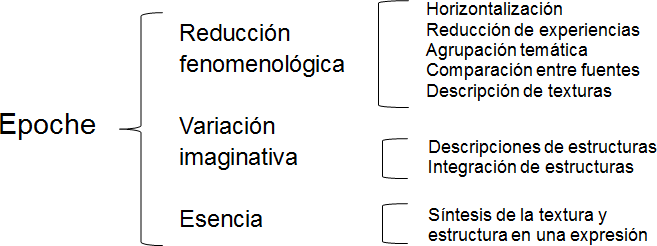
\includegraphics[width=\textwidth]{figura01.png}
\caption{El proceso de Epoche \cite{husserl_crisis_1970,moustakas_phenomenological_1994}.}
\label{Figura01}
\source{Elaboración propia.}
\end{minipage}
\end{figure}

En la variación imaginativa se derivaron temas estructurales a partir de las descripciones de las texturas obtenidas a través de la reducción fenomenológica y se comprendió que no existe una sola incursión a la verdad, sino que surgen innumerables posibilidades que están íntimamente conectadas con las esencias y significados de la experiencia. Por último, a través de la esencia se sintetizó la textura y la estructura en una expresión hasta conformar tres dimensiones y siete categorías. 

\section{Resultados y discusión}

Después de analizar los datos se presentaron tres dimensiones principales que incluyen categorías y subcategorías: a) implicaciones profesionales; b) implicaciones personales; c) pasión por la docencia (ver \Cref{Figura02}). En la siguiente sección se describen a detalle.

\begin{figure}[h!]
\centering
\begin{minipage}{.9\textwidth}
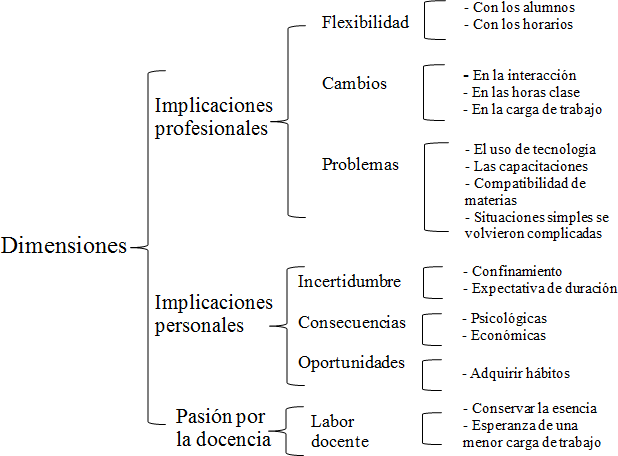
\includegraphics[width=\textwidth]{figura02.png}
\caption{Dimensiones, categorías y subcategorías.}
\label{Figura02}
\source{Elaboración propia.}
\end{minipage}
\end{figure}

\subsection{Primer dimensión: Implicaciones profesionales}

Esta dimensión resume los informes de los participantes respecto a las implicaciones profesionales que enfrentaron los profesores durante el confinamiento académico, entre los que destacan una modalidad más flexible, cambios en la práctica docente y algunas problemáticas.

Categoría: Flexibilidad.

Los profesores tuvieron que ser más condescendientes durante la modalidad virtual, se mantuvieron disponibles para sus estudiantes en horarios fuera de clase, inclusive los fines de semana y a altas horas de la noche. Con base en la respuesta de los participantes se encontraron dos subcategorías, las cuales fueron: \textit{flexibilidad con los alumnos y con los horarios}.

\textit{Flexibilidad con los alumnos}. Los profesores destacaron las adecuaciones que hicieron en su práctica docente para mostrarse flexibles con sus estudiantes al momento de asistir a clase, exponer, encargar tareas y realizar la evaluación del curso. Algunas respuestas se presentan a continuación.

\begin{quote}
Yo afortunadamente no he tenido hasta ahora situaciones de salud ni económicas mías o de mi familia, pero sé que muchos de mis estudiantes sí y entonces sé que eso implicó también que ellos se conectaran a última hora, que faltaran, se podría decir qué van poniendo en un segundo o tercer plano la educación. (María).

   Nunca sabes si se le fue el internet, si no tenía los recursos, “okey, no entregó, pero mira, te está diciendo que se fue la luz, bueno, dale chanza de un tiempito más, mira no puedes ser tan inflexible” porque tú mismo, en algunas capacitaciones me ha pasado “se me fue el internet” ¿Cómo voy a ser inflexible? (Román). 
\end{quote}

\textit{Flexibilidad con los horarios}. El tema del tiempo implicó la mayor muestra de flexibilidad por parte de los profesores, puesto que los alumnos los buscaban fuera del horario de clase, fines de semana e inclusive a altas horas de la noche para aclarar sus dudas. 

\begin{quote}
Los horarios de los alumnos y de uno varían, tienes que estar a la expectativa con relación a la hora que te manden el trabajo, pues no sabes si ellos se encontraron en un apuro o algo por el estilo, es complicado. (Omar).   
 
    Muchos alumnos me escribían a cualquier hora, cualquier día y era bastante frustrante, un sábado a las 11:50 de la noche “profe, es que tengo una urgencia” ¿si no le contesto? de todas formas me voy a quedar pensando, no voy a estar a gusto, no voy a saber qué. Y de hecho, mi esposo me decía “tú les contestas a cualquier hora, los malacostumbras” pero luego resultaba que sí estaban muy angustiados. (María).
\end{quote}

El contexto de la no presencialidad ha provocado que gran parte del profesorado aprenda sobre la marcha, desarrollando propuestas creativas e innovadoras para ajustar sus materiales, evaluaciones y formas de llevar a cabo la clase, lo que demuestra la capacidad de adaptación de los docentes \cite{penuelas_ensenanza_2020}, pero mientras los estudiantes valoran y agradecen esta flexibilidad, para los profesores representó un proceso agotador \cite{allen_teaching_2020}. Por lo anterior, es importante establecer acuerdos con los estudiantes respecto a las actividades a realizar y los horarios de las comunicaciones, con el objetivo de generar una conciencia sobre su responsabilidad y compromiso, para no abusar de la flexibilidad cuando los alumnos regresen a la modalidad presencial. 

Categoría: Cambios.

Para participar en la educación no presencial los profesores experimentaron importantes cambios, los principales estuvieron relacionados con las interacciones, puesto que gran parte de las relaciones interpersonales se redujeron quedando únicamente lo indispensable. Los horarios también se ajustaron, ya que algunas instituciones limitaron sus horas clase incorporando formatos sincrónicos y asincrónicos buscando aligerar la carga de los maestros. Sin embargo, a pesar de estas modificaciones los docentes expresaron un incremento en la carga de trabajo, ya que todas sus actividades, presentaciones y exámenes tuvieron que adaptarse a una nueva modalidad. Con base en la respuesta de los participantes se encontraron tres subcategorías de cambios, las cuales fueron: \textit{en la interacción, en las horas clase y en la carga de trabajo}.

\textit{En la interacción}. Las relaciones entre los docentes y alumnos cambiaron de manera significativa, la parte interpersonal se redujo al mínimo para únicamente conservar el contacto a través de medios electrónicos.

\begin{quote}
    Está bien cañón estarle hablando a una computadora y no ver a nadie, yo no les pido prender la cámara todo el tiempo porque el internet se hace más lento, entonces nadie pone la cámara, nada más la pongo yo y es bastante frustrante pues pareciera que estás hablando contigo misma. (Yessenia).
    
    Extraño el diálogo, la calidez de las personas, el compartir aula y el aprendizaje colaborativo, sin intentar forzarlo. Se fue haciendo este sentimiento entre el abandono y la ausencia, el sentir que todos están solamente escuchando lo que el maestro diga, se acaba la clase y se desconectan, se perdió la socialización. (María).
    
    Antes realmente se peleaban por participar, ahora los chicos eran como “caray, no participan” les da un pánico saber que se está grabando la sesión, equivocarse “qué van a decir los demás”. (Román).
\end{quote}

\textit{En las horas clase}. Algunas instituciones ajustaron los horarios de los docentes reduciendo las horas clase, a su vez, los profesores también combinaron clases sincrónicas y asincrónicas, ambas estrategias buscando hacer más llevadera la carga de trabajo.

\begin{quote}
  Empezando la pandemia nos dijeron que iba a ser muy pesado estar conectado todo el día, nos propusieron dejar una sola hora por cada tres, donde tenías que sintetizar mucho la información para abarcar todo. Tanto alumnos como maestros nos opusimos, pero al fin terminaron siendo hora y media para cada materia. (Armando).  

    Ya no nos podemos conectar las 4 horas, entonces dos sí nos conectamos y dos no, en las que no ahí meto las actividades que son como más de lectura y de escribir, y durante la clase la participación, para yo poder estar observando y coucheando. (Jazmín).

    Antes eran como dos horas clase, ahora una hora síncrona y una hora asíncrona. (Román).
\end{quote}

\textit{En la carga de trabajo}. A pesar de la reducción en las horas clase y la implementación de actividades de forma sincrónica y asincrónica, la mayoría de los profesores manifestaron sentir un incremento en la carga de trabajo.

\begin{quote}
    Para mí la verdad era demasiado trabajo. En mis presentaciones buscar esas imágenes que van a transmitir lo que tú quieres, el mismo tipo de letra, estar justificadas, no poner tantos colores, pero sí que pueda diferenciarse con los del fondo. En lugar de llevarme una hora preparar la clase, ahora se puede llevar hasta dos, a pesar de que son más cortitas. (Armando).

    Se ha incrementado la cantidad de trabajo, yo ya tenía todo diseñado para la clase y al hacerlo en línea, pues tuve que hacer muchos cambios, por ejemplo, los examencitos que les ponían mis alumnas, pues antes imprimía un Word que ya tenía hecho y se los daba, y ahora es pasarlo a un medio electrónico, ahora también subir las tareas a la plataforma, cosas que antes no hacía. (Diana).

    Siguen siendo las mismas horas, pero la cuestión de programar una clase en línea, estar al tanto de calificaciones y todo siento que me volvió un poco más productivo, el grado de exigencia fue mayor, me sentía con más trabajo. (Tadeo).
\end{quote}

Sin tiempo para adaptarse y realizar una planificación adecuada, los centros educativos se enfrentaron al reto de continuar impartiendo sus cursos en una modalidad no presencial implementando tecnologías \cite{donitsa-schmidt_opportunities_2020}, donde, a pesar de todas las herramientas de comunicación disponibles, las interacciones fueron limitadas y prevaleció una sensación de abandono. Otros de los cambios fueron la reducción de las horas clase y la incursión de un formato sincrónico y asincrónico, sin embargo, a pesar de que estas modificaciones tenían el objetivo de limitar el tiempo que los docentes estaban frente al grupo, la preparación de los contenidos muchas veces requería más esfuerzo, al ser un cambio repentino implicó un aumento en el tiempo destinado a la creación de los materiales, resultando en una mayor carga de trabajo que no estaba contemplada \cite{penuelas_ensenanza_2020}. 

Categoría: Problemas.

Transitar a una modalidad virtual no fue una tarea fácil y los docentes enfrentaron varias dificultades, las primeras complicaciones estuvieron relacionadas con el uso de la tecnología, aunque continuamente se incorporan herramientas tecnológicas a los salones de clases, las habilidades de los profesores en su uso son limitadas. Además, cuando las instituciones implementaron cursos y capacitaciones para su personal, en lugar de ser vistas como un apoyo eran consideradas un obstáculo al ser muy básicas, consumirles tiempo fuera de su horario laboral y no ser remuneradas. Por otra parte, no todas las materias eran compatibles con esta modalidad, ya que aquellas que requerían un trabajo menos teórico y más práctico se complicaban por el confinamiento. Finalmente, situaciones pedagógicas o administrativas que se resolvían fácilmente en la modalidad presencial se dificultaban en lo virtual. Con base en la respuesta de los participantes se encontraron cuatro subcategorías, las cuales fueron: \textit{el uso de tecnología, las capacitaciones, compatibilidad de materias y situaciones simples se volvieron complejas}.

\textit{El uso de tecnología}. Aun cuando las herramientas tecnológicas se utilizan frecuentemente en los salones de clases, algunos profesores tienen conocimientos muy básicos o prefieren usar metodologías tradicionales, lo que se ve reflejado en su falta de habilidades. Por otra parte, al estar tanto alumnos y docentes desde sus casas aparecieron otros problemas relacionados con la infraestructura como son fallas en los dispositivos o problemas de conexión a internet.

\begin{quote}
    Tenemos una plataforma, ya existía una herramienta para impartir clase a los alumnos, pero es tanta la costumbre a lo presencial, también la mayoría de los maestros eran mayores y casi no usaban la tecnología. No tuvimos la precaución de familiarizarnos con estas plataformas, porque pensábamos que nunca iba a llegar a pasar algo así. (Omar).

    Muchos alumnos son “mi cámara no sirve, es que mi micrófono no sé qué”, hay otros que me han dicho “no tengo internet, ya se me van a acabar los datos y se va a cortar la clase”. (Yessenia).

    Algo que me ha tocado infinitamente es que a veces se caen las redes de internet. (Diana).
\end{quote}

\textit{Las capacitaciones}. Contrario a lo que podría pensarse, las capacitaciones fueron ampliamente mencionadas por los docentes como una fuente de problemas, los profesores no las ven como la mejor opción para adquirir conocimiento, sino como una alternativa que aporta recursos muy generales que no están enfocados a su práctica diaria, además les quita tiempo y por si fuera poco no es remunerado.

\begin{quote}
    En la universidad estuvieron cambiando muchas veces de plataformas, estuvimos usando Moodle, Teams, Zoom, sí nos capacitaron, pero era otra hora extra a lo que es tu trabajo y a veces en fin de semana, creo que fue un poquito tedioso, una plataforma y luego otra. (Armando).

    Lo viví en un bombardeo de información, para mí fue un poquito pesado porque eran capacitaciones de varias instituciones. (María).

    Tuve que ir a capacitaciones que no quería, soy muy autodidacta y me desesperaba mucho que nos metieron a todos los profes a tomar el curso en tal cosa, cuando pudieron haber hecho una evaluación de ver qué profe lo necesitaba, para que pudiera yo tener capacitaciones que se adaptaran a mis objetivos. Son capacitaciones que no se te pagan y digamos que me agarré unos ciertos corajes institucionales. (Román).
\end{quote}

\textit{Compatibilidad de materias}. Los docentes hicieron énfasis en la incompatibilidad de algunas materias con la modalidad virtual, mientras que para los contenidos teóricos fue una transición sencilla, las unidades más prácticas tuvieron bastantes dificultades. 

\begin{quote}
    En las mías es más teoría, se acomodan súper bien para que sean en línea, sobre todo porque son estructuras cerebrales, uno no puede abrirse la cabeza y mostrar, sino más bien tiene que utilizar imágenes, imágenes, imágenes. (Armando).

    Tengo materias de prácticas donde tienen que trabajar con niños, entonces es bien difícil tener un horario compatible con el niño y con los papás, para que el papá pueda para hacer la videollamada y que se pueda ver al niño, luego aparte mis alumnos tienen que entrenar o capacitar a los padres para que le pongan la actividad y ellos puedan estar observando a distancia y pues igual, no observas bien. (Yessenia).

    Muchas cosas se pueden adaptar, pero sí tenemos muchas limitaciones, por ejemplo, en estos días toca hacer una disección y pues no sé cómo le vamos a hacer, porque tienes que hacerlo, al menos si te da asco el cerebro lo ves aunque no participes, pero vamos al laboratorio, te pones tu bata y todo, este tipo de experiencias muy vivenciales. (Cesar).
\end{quote}

\textit{Situaciones simples se volvieron complicadas}. Los profesores también manifestaron que situaciones que fácilmente solucionaban dentro del formato presencial se volvieron de difícil respuesta en el entorno virtual, esto aplicó para actividades dentro del salón de clases tales como debates, la revisión de tareas o brindar una asesoría, así como complicaciones en cuestiones administrativas al solicitar trámites y servicios. 

\begin{quote}
    Cuando estás en presencial das indicaciones e invitas a los alumnos a participar, ahora es un poquito difícil porque aunque digas los nombres todos quieren participar, y es difícil si proyectas alguna imagen o actividad estar poniendo atención al grupo, porque te muestra unas cuantas pantallitas, entonces quieren hablar al mismo tiempo y eso como que retrasa la clase. (Omar).

    Es típico “necesito información de no sé qué, hay que mandar un correo a fulanito, es que no me contesta, bueno mándaselo a zutanito, es que él me dijo que no se encarga de eso” cosas que tú podías hacer caminando al departamento de X o Y persona para tener respuesta, ahora es como que entre los chorrocientos mil mails y a ver si no le llegan al correo basura, para que me resuelvan algo mínimo. (Tania).

    Yo quería ser como en lo presencial “si mira, a ver” no me toma tiempo, porque era ahí mismo, mientras trabajan los demás separaba al chico que tenía dudas y ya en privado le respondidas, pero acá era “se me fue la luz, qué hicimos el día de hoy profe”. (Román).
\end{quote}

Entre las principales dificultades para convertir sus cursos tradicionales a la modalidad no presencial está el uso de la tecnología, ya que muchos maestros reconocen una escasa preparación en ambientes virtuales de aprendizaje, por lo que se han programado gran cantidad de seminarios de formación \cite{penuelas_ensenanza_2020}. Sin embargo, un exceso en las capacitaciones representa un problema para los maestros, porque incluyen contenidos muy generales, consumen una amplia cantidad del tiempo de los docentes y no son remuneradas. Otro problema es la incompatibilidad de materias, puesto que aunque los profesores consideran que todo se puede adaptar, las unidades de aprendizaje que implican observación, entrevistas o manipulación de dispositivos tienen un mayor grado de complejidad, inclusive, tareas sencillas como un debate o una sesión de preguntas y respuestas tienen sus complicaciones \cite{van_nuland_covid-19_2020}. Por lo anterior, sería necesario orientar la formación de los maestros por niveles de acuerdo con los conocimientos que ya tienen en el uso de recursos digitales y que las capacitaciones se lleven a cabo dentro de su jornada laboral. Además, en el regreso a las aulas se deben priorizar las materias de prácticas o laboratorios, ya que a diferencia de las teóricas presentan dificultades para realizarse en entornos virtuales.  

\subsection{Segunda dimensión: implicaciones personales}

Esta dimensión resume los informes de los participantes respecto a las implicaciones personales que tuvieron que enfrentar los profesores por la vida en confinamiento, destacando sus primeras reacciones, los cambios en sus hábitos, la expectativa de duración, los efectos psicológicos, el impacto económico y algunas oportunidades presentadas.

Categoría: Incertidumbre.

La pandemia por la Covid-19 generó una gran incertidumbre en la vida personal de los docentes, a pesar de que sus consecuencias ya estaban presentes en otras partes del mundo sus alcances aún eran desconocidos. Las medidas de sana distancia fueron puestas en marcha como una manera de contener el virus y aunque las expectativas de duración del confinamiento eran positivas, la realidad fue totalmente distinta y los maestros tuvieron que acostumbrarse al encierro por un largo periodo. Con base en la respuesta de los participantes se encontraron dos subcategorías, las cuales fueron: \textit{confinamiento y expectativa de duración}.

\textit{El Confinamiento}. Los profesores tuvieron que adaptarse a las políticas de distanciamiento social, reduciendo al mínimo su contacto con otras personas, dejando de hacer actividades cotidianas y de recreación.

\begin{quote}
    Dejé de ir a reuniones familiares, de amistades, fiestas, salir de compras, andar de rol. Incluso también dejé de ver a mi novia un tiempo, porque teníamos que estarnos guardando los primeros meses y pues ya poco a poco nos fuimos viendo. (Omar).
    
    Yo creo que la que más me dolió fue el ejercicio, porque iba a diario al gimnasio de la universidad después del trabajo, pero pasó lo de la contingencia y todos los gimnasios cerraron. Empecé a dejar esa rutina que me gustaba mucho y después fue como “oye puedes hacer ejercicio en casa” pero no es lo mismo, aun cuando te mates todo el día, no es lo mismo, no es la cuestión de los aparatos, también es el ambiente, la convivencia que hay dentro del gimnasio, o sea, no la tienes en casa. (Tadeo).
    
    El hecho de salir a correr, hubo un tiempo que ni siquiera podía salir al parque o a la calle, a una plaza simplemente a caminar, a ver otras caras, fui reduciendo un poco el tiempo en el que lo hacía. (Jazmín).
\end{quote}

\textit{La expectativa de duración}. Una vez que se implementó el confinamiento los docentes tenían expectativas muy positivas en relación con su duración, en parte por su experiencia con el virus de la influenza Ah1n1, sin embargo, con el paso de los meses y el relajamiento de las medidas de sana distancia vieron cada vez más distante el regreso a la normalidad.

\begin{quote}
    ¡Ay! Yo pensé que iban a durar como dos meses, pero también había escuchado que podía tomar de que 3 años o así. (Tania).

En un inicio pensé que ya para septiembre íbamos a regresar a la normalidad, conforme avanzó esto ya me había hecho a la idea que hasta el 2021 vamos a regresar. Ahora creo que va para largo. (Diana).

Al principio sí pensé que sería como un mes de confinamiento y cuando pasó el mes me generó esa incertidumbre, ahorita te digo que no sé cuándo vaya a ser el regreso. (Cesar).
\end{quote}

La declaración de la Covid-19 como una pandemia por la OMS produjo una crisis en la salud y economía a nivel global \cite{world_health_organization_coronavirus_2020}. En respuesta, las políticas de distanciamiento social obligaron a las personas a resguardarse en sus hogares, estimulando nuevas formas de establecer relaciones de trabajo, ocio y educación \cite{valle_martinez_experiencia_2020}. En un inicio, la respuesta de los profesores fue de incertidumbre puesto que poco se conocía del virus y aun cuando se adoptaron las medidas del confinamiento, las expectativas de duración de la pandemia eran muy positivas. Sin embargo, posteriormente cayeron en cuenta que el regreso a la normalidad no será una simple transición a la vida como solía ser \cite{daniel_education_2020}, sino que se tendrían que adoptar algunos protocolos de higiene y prepararse para una nueva realidad.

Categoría: Consecuencias.

De esta forma, el confinamiento tuvo fuertes repercusiones en la vida personal de los docentes, mientras que las psicológicas incluyeron algunos sentimientos negativos y desesperanza, con el pasar de los meses aprendieron a controlar estas emociones y se enfocaron en lo positivo. Por su parte, en el aspecto económico algunos profesores obtuvieron bonos, redujeron sus gastos o no fueron afectados, mientras que otros vieron disminuidos sus sueldos, incrementaron sus gastos en el hogar o inclusive dejaron de percibir ingresos de otras fuentes. Con base en la respuesta de los participantes se encontraron dos subcategorías relacionadas con las consecuencias, las cuales fueron: \textit{psicológicas y económicas}.

\textit{Psicológicas}. Los docentes expresaron sentimientos negativos como estrés, ansiedad y miedo, sobre todo en las primeras semanas del confinamiento debido a la incertidumbre y el desconocimiento del virus, sin embargo, con el paso del tiempo fueron capaces de controlar esas emociones y se enfocaron en los aspectos positivos. 

\begin{quote}
    Yo he tenido todos los episodios, primero ansiedad de si salía me iba a pasar algo y entonces vamos a lavarnos las manos. Después, pasar tanto tiempo con las mismas personas era insoportable, me acuerdo al principio videollamadas con amigos y todo, también la etapa de hacer un chorral de ejercicio, después no hacía nada y luego solo comer. Tener que vivir un año de tanta enfermedad y muertes sí te pega, sobre todo pensando en mis papás, en mis abuelos, en todo eso, ha sido como muy fuerte. (Yessenia).
    
    Era muy triste, muy deprimente, el sentir que ya no había mucho control sobre las cosas, porque ya no puedes comer afuera, ya no puedes salir con tus amigos. (Tania).
    
    Yo creo que a mitad del año sí me pegó, los primeros meses fue de que “Ah, pues bien, en casa a gusto” yo era una persona que salía mucho en fines de semana y a mitad de año empecé a extrañar todo eso y fue como “necesito salir, quiero salir, pero no puedo salir”, sí me pegó, no puedo decir que fue depresión ni nada, pero sí me encontré como en una especie de ansiedad. (Tadeo).
\end{quote}

\textit{Económicas}. El confinamiento tuvo un impacto económico en los docentes, mientras para algunos fue positivo por la obtención de estímulos o la reducción de gastos, para otros fue negativo por la rebaja de sueldos, el incremento de consumos en el hogar o la pérdida de otras fuentes de ingresos. 

\begin{quote}
    Me afectó económicamente, el rector habló con nosotros “vamos a tener que evitar bajas y que los alumnos continúen estudiando, vamos a bajar las colegiaturas y los sueldos de maestros” y esto era alrededor del 30 \%, entonces se iban a incrementar los tiempos de labor, pero con menos paga. Incluso hay algunas aplicaciones que requieren una membresía donde uno tiene que invertirle para poder tener una mejor calidad de enseñanza, sí nos afectó en cuestiones económicas. (Omar).
    
    Los gastos de la casa han aumentado, estoy conectada todo el día, la luz, el aire acondicionado, el internet tuvimos que subirlo a uno más rápido, la comida al estar todo el día en casa, aquí desayuno, como, ceno. Aparte tenía muchos proyectos sociales de trabajar en las comunidades y como están detenidos me han pegado en el bolsillo. (Yessenia).
    
    Me están dando un bono por la  COVID, yo creo que a lo mejor puede ser por la institución donde estoy, como es un área clínica, muchas veces tengo que ir y los alumnos igual. (Diana).
\end{quote}

El confinamiento por la pandemia de la Covid-19 tuvo consecuencias negativas en los docentes, además de la incertidumbre y el estrés que se generó por la falta de información, se aunaron también sentimientos de irritabilidad, enfado, angustia, miedo, ansiedad y problemas de sueño como consecuencia de la vida en confinamiento \cite{quispe_victoria_impacto_2020}, este malestar general se manifestó sobre todo en los primeros meses del encierro, pero con el paso del tiempo los profesores supieron sobrellevarlo. No obstante, además del desgaste físico y emocional que implicó la migración al formato en línea, varios docentes vieron afectada su economía, unos por reducciones de sueldo a pesar de estar dedicando más tiempo a su trabajo \cite{penuelas_ensenanza_2020}, otros incrementaron sus gastos al estar en casa pero no sus ingresos, mientras que algunos perdieron proyectos que representaban otra fuente de dinero.

Categoría: Oportunidades.

A pesar de las consecuencias negativas de la vida en confinamiento, también se presentaron importantes oportunidades para los docentes como lo son adquirir hábitos más saludables o retomar pasatiempos, así como aprovechar al máximo los conocimientos adquiridos para una modalidad digital. Con base en la respuesta de los participantes se encontró una subcategoría, la \textit{oportunidad de adquirir hábitos}.

\textit{Adquirir hábitos}. Aunque fue difícil respetar las políticas de distanciamiento social en un inicio, una vez que los profesores universitarios se acostumbraron al encierro tuvieron oportunidad de utilizar la mayor cantidad de tiempo disponible para cuidar su alimentación, hacer ejercicio, tomar cursos de formación y realizar otras actividades agradables para ellos.

\begin{quote}
    Ahora soy un poco más organizado, estoy tratando de hacer más de ejercicio, también de las compras ni se diga, ¡Amazon no te acabes! Me compré un búho grande para pintarlo, entonces cuando estoy muy cansado por algo me pongo a pintar. (Armando).
    
    Corro todos los días, nada más siento que va aumentando el estrés y me subo a la caminadora, empecé a tomar en cuenta cosas en mi casa, como regar las plantas. (Tania).
    
    He estado haciendo ejercicio y poniendo más cuidado en mí, ver Netflix, jugar un videojuego, cosas que antes eran muy difíciles porque me faltaba el tiempo y ya no quería hacer nada, ahora creo que le pongo un poco más de entusiasmo a lo personal. (Cesar).
\end{quote}

A pesar de las implicaciones negativas debidas al confinamiento en su vida personal, los docentes tuvieron oportunidad de enfocarse más en ellos, hacer actividades que antes eran imposibles por el tiempo, retomar antiguas aficiones y adquirir conductas de salud como lo son hacer ejercicio y cuidar su alimentación, inclusive, desean conservar estos nuevos hábitos cuando regresen a la modalidad presencial. Sin duda esto se verá reflejado en los sistemas educativos, se espera que experimentar un enfoque con tantas oportunidades produzca un cambio crítico en un futuro próximo, esta pandemia será recordada como una etapa de aprendizaje en la cual los profesores no solo adquirieron habilidades para aplicar dentro de los salones de clases, sino también hábitos en su vida cotidiana \cite{burgos_6-key_2021}.

\subsection{Tercer dimensión: pasión por la docencia}

Esta dimensión resume los informes de los participantes respecto a cómo reafirmaron su pasión por la docencia durante la migración a la educación no presencial, aquellos elementos que tuvieron que incorporar en la nueva modalidad, la esencia que conservaron de lo tradicional y la esperanza de un futuro alentador. 

Categoría: Labor docente.

Los profesores destacaron la importancia de su esfuerzo en una nueva modalidad, qué ajustes tuvieron que realizar, cuáles fueron sus motivaciones y cómo pueden transformar la vida de sus alumnos convirtiéndose en una fuente de inspiración. Aunque los maestros aceptan que la nueva modalidad requirió una gran cantidad de trabajo, también reconocen que este puede ser reutilizado de una forma más sencilla. Con base en la respuesta de los participantes se encontraron dos subcategorías, las cuales fueron: \textit{conservar la esencia y esperanza de una menor carga de trabajo}.

\textit{Conservar la esencia}. Para desempeñarse en una modalidad virtual los docentes tuvieron que hacer ajustes en su forma de trabajar, sin embargo, siempre trataron de conservar su esencia, aquello que los caracterizaba en la modalidad presencial y era reconocido por sus estudiantes. 

\begin{quote}
    Trato de conservar la parte de la relación, ser muy cercana con mis alumnos, siempre dar unos minutitos para hablar de cómo están, cómo se sienten, cómo les ha ido, qué dificultades han tenido o tocar situaciones que se han presentado en su trabajo en el departamento, eso es algo que he tratado de continuar haciéndolo, no volverlo tan impersonal como puede llegar a ser un medio virtual. (Diana).
    
    La parte de la empatía creo que sí se pudo acomodar, el hecho de hacer un poco de rapport al inicio “cómo les va” “qué saben de lo nuevo”. Los alumnos inclusive lo externaron en juntas y ahora otros maestros dedican unos minutos a la misma actividad. (Jazmín).
    
    He conservado mi frase de bienvenida al iniciar, sigo incorporando videos y sigo manteniendo mi retroalimentación, pero ahora virtual, en algún punto yo me iba a otro canal o visitaba a cada uno de los equipos, me gustó mucho cómo funciona eso. (Román).
\end{quote}

\textit{Esperanza de una menor carga de trabajo}. Aunque los docentes reconocen la gran cantidad de trabajo que implicó la migración a un formato digital en un inicio, también son conscientes que los recursos que están creando pueden ser reutilizables y a la larga se pueden traducir en una menor cantidad de trabajo. 

\begin{quote}
    Eso de preparar los materiales siento que ya pasó, casi todo ya lo tengo hecho, ahora solamente me pongo a releer para antes de la clase y a modificar algunos detalles. (María).
    
    El primer tetra fue muy pesado y después ya tenía todo totalmente hecho, como eran las mismas materias, solamente iba cargando la misma información. (Jazmín).
    
    Creo que todo se puede ajustar para que sea menos trabajo, tengo la fiel convicción de que a pesar de que fue mucho trabajo para mí, gran parte implicó el proceso de adaptación, sí creo que va a ser menos trabajo a la larga en cuanto termine de mostrarle a los alumnos cómo hacerles la vida más sencilla para hacerme la vida más sencilla. (Román).
\end{quote}

Aunque la pandemia develó problemáticas de acceso y manejo de tecnologías digitales, eso no fue impedimento para que los docentes continuaran transmitiendo su esencia durante las clases, de hecho, el regreso a las aulas representa un espacio para aprovechar las herramientas tecnológicas y los conocimientos que potenciaron los profesores en el marco de la innovación educativa \cite{valle_martinez_experiencia_2020}. Además, este tipo de crisis permite a la sociedad dimensionar la importancia del trabajo de los profesores y valorar su papel imprescindible dentro de la comunidad. El siguiente desafío para los maestros es fortalecer y consolidar todos los cambios en su práctica docente para dar respuesta efectiva ante los retos del futuro de la educación \cite{donitsa-schmidt_opportunities_2020}.

\section{Conclusiones}

Este estudio investigó de forma exploratoria el impacto del confinamiento académico desde la perspectiva de docentes jóvenes y universitarios, producto de la pandemia por la Covid-19. Los datos sugieren que la nueva modalidad de enseñanza presentó diversos desafíos para los profesores, quienes tuvieron que hacer ajustes en su práctica docente para transitar a entornos virtuales. Mientras que los cambios se realizaron principalmente en el terreno profesional, algunas repercusiones alcanzaron también el ámbito personal, destacando las implicaciones psicológicas y económicas del confinamiento, sin embargo, también se presentaron oportunidades. Otro punto interesante fue la facilidad con que los profesores se adaptaron al uso de la tecnología durante el periodo de emergencia sanitaria y cómo se prepararon para el siguiente ciclo escolar declarado confinado, quizá esto se deba a la edad de los docentes, habría que analizar esta variable con otro rango de edad de los profesores. Por último, la pasión por la docencia emerge como un elemento que potencia el esfuerzo y la disposición de los profesores para continuar con la enseñanza a pesar de las condiciones y revalora su papel como pilares dentro de la sociedad. 

Entre las limitaciones de este estudio está que los participantes se extrajeron de una muestra de conveniencia y las posibilidades de generalización son limitadas, no obstante, se cuidó la variabilidad de los profesores, tanto en su género, edad y tipo de institución. Los hallazgos del estudio pueden verse como una construcción desde los docentes, la literatura, así como de los investigadores que pretenden expresar el sentir de los participantes.

Es necesario continuar la investigación para ampliar el conocimiento sobre las implicaciones del confinamiento en los docentes universitarios. Invitar a estudiantes y directivos permitiría saber cómo otros involucrados en el proceso de enseñanza y aprendizaje perciben a los profesores. Además, incorporar técnicas de observación participante o no participante sería también de utilidad. Finalmente, con el retorno a las aulas se podría continuar la investigación para conocer qué cambios adoptados para la migración a un formato virtual permanecieron al regreso de la modalidad presencial.


\printbibliography\label{sec-bib}
% if the text is not in Portuguese, it might be necessary to use the code below instead to print the correct ABNT abbreviations [s.n.], [s.l.]
%\begin{portuguese}
%\printbibliography[title={Bibliography}]
%\end{portuguese}


%full list: conceptualization,datacuration,formalanalysis,funding,investigation,methodology,projadm,resources,software,supervision,validation,visualization,writing,review
\begin{contributors}
\authorcontribution{Francisco Javier Rocha Estrada}[conceptualization,datacuration,formalanalysis,methodology,validation,visualization,writing,review]
\authorcontribution{Elvira Guadalupe Rincón Flores}[conceptualization,methodology,writing,review]
\end{contributors}

\appendix
\section{Apéndice: Guía de entrevista}\label{Anexo}

Iniciar preguntas de rapport. 

Informar la confidencialidad de la información, la participación libre y voluntaria.

¿Cuántas horas clase impartes a la semana?

¿Cuántos años tienes de experiencia impartiendo clases en nivel superior?

Cuando te notificaron la suspensión de clases por la pandemia ¿Qué fue lo primero que pensaste?

¿Tu universidad tenía modalidad en línea?

¿Consideras que tu materia es compatible con las clases en línea?

Al saber que regresarían las clases en la modalidad en línea ¿Tuviste alguna iniciativa para empezar a conocer las nuevas herramientas tecnológicas que utilizarías en tus clases?

En un inicio ¿Cuánto tiempo pensaste que durarían las clases en línea?
¿Qué características has conservado de tu práctica docente presencial al migrar al formato en línea? ¿Cuáles no has conservado? ¿Qué otras has adquirido?

Descríbeme ¿Cómo eras como docente presencial? ¿Qué te caracterizaba?

Descríbeme ¿Cómo eres como docente en línea?

¿Te veías hace un año dando clases en línea?

¿Qué es lo que más te gusta de dar clases en línea?

¿Qué extrañas de las clases presenciales?

¿Consideras que ha cambiado tu carga de trabajo?

¿Este cambio en la modalidad ha tenido un impacto económico en tu vida?

¿Qué significa para ti continuar con tu labor docente a pesar de la pandemia? 

En comparación con las primeras semanas de la cuarentena ¿cómo te sientes actualmente?

¿Cuál ha sido el impacto psicológico que has tenido por el confinamiento?

¿Qué actividades dejaste de realizar?  ¿Qué nuevos hábitos has adquirido?

¿Cuándo crees que esto termine? ¿Cómo crees que será la nueva normalidad?

¿Qué ha sido para ti lo más difícil de este cambio en el ámbito profesional y personal?


\end{document}

